\documentclass[numbers=noenddot,12pt,a4paper]{scrartcl}
\usepackage[greek,ngerman]{babel}
\usepackage[T1]{fontenc}
\usepackage[utf8]{inputenc}
\usepackage{fullpage}
\usepackage{libertine}
\usepackage{ziffer}
\usepackage{graphicx}
\usepackage{units}
\usepackage[infoshow]{tabularx}
\usepackage{amsmath}
\usepackage{amssymb}
\usepackage{wrapfig}
\usepackage{esint}
\usepackage{float}
\usepackage{wrapfig}
\usepackage[font=small]{caption}
\usepackage{subcaption}
\usepackage{lscape}
\usepackage{hyperref}

\renewcommand{\thefigure}{Abb. \arabic{figure}}

\captionsetup[wrapfigure]{name=}
\captionsetup[figure]{name=}
\newcommand{\nummat}[1]{\left[\text{#1}\right]}
\newcommand{\num}[1]{$\left[\text{#1}\right]$}
\newcommand{\degree}{^\circ}
\newcommand{\diff}{\textnormal{d}}
\newcommand{\tenpo}[1]{\cdot 10^{#1}}
\newcommand{\greek}[1]{\greektext#1\latintext}
\newcommand{\ix}[1]{_\text{#1}}
\newcommand{\imag}{\mathbf{i}}
\newcommand{\tilt}[1]{\textit{#1}}
\newcommand{\grad}[1]{\textit{grad}\left(#1\right)}
\newcommand{\divergenz}[1]{\textit{div}\left(#1\right)}
\newcommand{\euler}{\mathnormal{e}}
\newcommand{\fett}[1]{\textbf{#1}}

\title{Protokoll: Myonenspektrometer} %TODO Name des Versuchs eintragen
\author{Philipp Hacker} %TODO Protokollschreiber unterstreichen
\date{\today}

\begin{document}
%\setcounter{page}{2}
%\setcounter{section}{1}
\maketitle
\begin{center}
Betreuer: Prof. Dr. R. Hippler \\ %TODO Name des Betreuers eintragen
Versuchsdatum: 16./17./18.12.2014\\ %TODO Datum des Versuchs eintragen
\begin{table}[h]
\centering
Note: %TODO Gute Note erhalten :)
\begin{tabularx}{1.5cm}{|X|}
\hline \\ \\
\hline
\end{tabularx}
\end{table}
\end{center}
\vspace*{\fill}
\tableofcontents
\vfill
\newpage
\section{Einleitung}
Das Myon $\mu\pm$ wurde 1936 von C.D. Anderson und S. Neddermeyer während der Untersuchung kosmischer Strahlung entdeckt. Es ist ein Zerfallsprodukt dessen, welcher unter Wechselwirkung mit unserer Atmosphäre hervorgerufen wird. Heute können sie künstlich in Teilchenbeschleunigern erzeugt werden. Sie gehören, genau wie das stark ähnelnde, jedoch viel leichtere Elektron, zu den Leptonen. Ihre Beobachtung auf der Erdoberfläche kann als Bestätigung der relativistischen Zeitdilation angesehen werden. Ihre Lebensdauer allein würde, selbst beim Abstieg aus der oberen Atmosphäre mit Lichtgeschwindigkeit, nicht ausreichen, damit wir sie mit einfachen Mitteln im Labor messen könnten.\\
In diesem Versuch soll gerade diese Zeit gemessen werden. Weiterhin werden statistische Aussagen über den Zerfall und den Myonen-Strom aus der Atmosphäre gemacht. Dafür wird im Folgenden auf die Wechselwirkung dessen mit Materie und die grundlegenden Prinzipien der Myonenspektrometrie eingegangen.
\newpage
\section{Grundlagen}
\subsection{Entstehung und Zerfall von Myonen}
\begin{wrapfigure}[15]{ro}{0.4\textwidth}
	\centering
	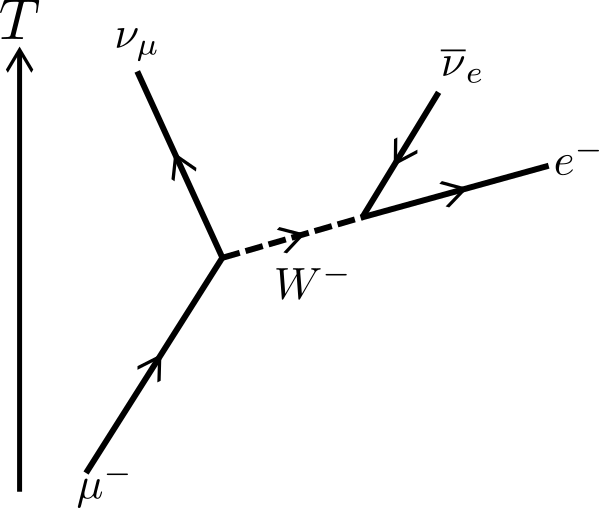
\includegraphics[width=0.4\textwidth]{Muon_Decay.pdf}
	\caption{Feynman-Diagramm des Zerfalls eines $\mu^-$}\label{img:zerfall}
\end{wrapfigure}
Durch die \tilt{primäre kosmische Strahlung} wird die Atmosphäre der Erde mit, größtenteils schweren Partikeln beschossen. Diese sind in der Regel Protonen und $\alpha$-Teilchen, können jedoch auch große Nuklide sein. Dieser Schauer aus schweren Teilchen wechselwirkt mit den Molekülen der Erdatmosphäre und zerfällt dabei, gegebenenfalls in mehreren Schritten, kaskadierend in seine Bestandteile. Das Zwischenprodukt der kosmischen Strahlung enthält, unter Anderem, Protonen, Pionen, Neutronen, Kaonen, Photonen, Elektronen und Positronen.\\
Das zu untersuchende Teilchen in diesem Versuch ist das Myon $\mu^\pm$. Dessen Flussdichte liegt bei etwa $\unit[100]{\frac{1}{m^2\cdot s}}$. Es gehört zu den Leptonen und ist einfach positiv bzw. negativ geladen (Anti-/Myon), wobei das Verhältnis $\mu^+/\mu^-=1,27$ beträgt. Es ist in seinen Eigenschaften vergleichbar mit dem Elektron: es besitzt einen Spin von $1/2$ und unterliegt nur der elektroschwachen, nicht jedoch der starken Wechselwirkung. Im Unterschied zum $e^-$ ist jedoch seine Masse um etwa das 200-fache größer und es besitzt nur eine mittlere Lebensdauer von $\unit[2,196\cdot 10^{-6}]{s}$. Der Fakt, dass wir trotzdem in der Lage sind, das Myon, welches in einer Höhe von rund $\unit[10]{km}$ in der oberen Atmosphäre entsteht, an der Erdoberfläche zu messen, ist Folge der relativistischen Zeitdilatation bewegter Inertialsysteme.\\
Das gesuchte Teilchen entsteht zusammen mit einem Anti-/Neutrino aus dem spontanen Zerfall eines Pions $\pi^\pm$ (Gl. (\ref{eq:plus}), (\ref{eq:minus})).
\begin{align}
\pi^+\rightarrow&\mu^++\nu_\mu \label{eq:plus}\\
\pi^-\rightarrow&\mu^-+\overline{\nu}_\mu \label{eq:minus}
\end{align}
Die freien Myonen zerfallen nun mit hoher Wahrscheinlichkeit, unter Verlust ihrer kinetischen Energie, in ein Elektron/Positron und 2 jeweilige Anti-/Neutrinos.
\begin{align}
\mu^+\rightarrow& e^++\nu_e+\overline{\nu}_\mu \label{eq:eins}\\
\mu^-\rightarrow& e^-+\nu_\mu+\overline{\nu}_e\label{eq:zwei}
\end{align}
\ref{img:zerfall} zeigt das Feynman-Diagramm des Zerfalls des Antimyons in ein Myonenneutrino, Elektronenantineutrino und Elektron. Dabei überträgt das negativ geladene Elementarteilchen des $W^-$-Bosons$^{\nummat{II}}$ die elektroschwache Wechselwirkung, welche zur Erzeugung des Elektron-Antineutrino-Paares nötig ist.
\newpage
Außerdem ist es möglich , dass der Myonen-Zerfall Photonen (Gl.(\ref{eq:phot})) aussendet (Wahrscheinlichkeit $1,4\%$)$^{\nummat{I}}$, oder ein Elektron-Positron-Paar (Wahrscheinlichkeit $3,4\cdot10^{-3}\%$)$^{\nummat{I}}$ erzeugt (Gl. (\ref{eq:elekpos}).
\begin{align}
	\mu^-\rightarrow e^-+\overline{\nu}_e+\nu_\mu+\gamma \hspace{2cm} \mu^+\rightarrow e^++\nu_e+\overline{\nu}_\mu+\gamma \label{eq:phot}\\
	\mu^-\rightarrow 2e^-+e^++\overline{\nu}_e+\nu_\mu \hspace{2cm} \mu^+\rightarrow e^-+2e^++\nu_e+\overline{\nu}_\mu \label{eq:elekpos}
\end{align}
Mit einer zu $Z^4$ proportionalen Wahrscheinlichkeit, wobei $Z$ die Kernladungszahl ist, kann ein negatives Myon mit einem Atom, unter Einfang eines Elektrons der K-Schale, ein \tilt{myonisches Atom} bilden und dadurch in das Nuklid eingezogen werden. Die damit ausgelöste Umwandlung eines Protons in ein Neutron findet unter Emission eines $\nu_\mu$ statt. Die Zeit dieses Vorgans ist klein gegen die Lebensdauer des $\mu^-$, jedoch ergibt die Messung in Materie eine Zerfallszeit von Myonen, welche kleiner als die, der im Vakuum gemessenen Zerfälle ist. Die Halbwertszeit positiver Myonen ist offensichtlich damit größer, da für sie kein zusätzlicher Zerfallskanal besteht.\\
Unter spontanem Zerfall folgt die Zahl $N$ der Myonen Gl. (\ref{eq:zerfall}). Dabei ist die Anzahl $N\ix{0}$ zu einer Zeit $t\ix{0}$ bekannt. Die Zerfallsrate $\lambda$ lässt sich außerdem in die mittlere Lebensdauer, oder auch Halbwertszeit $\tau=1/\lambda$ überführen und umgekehrt.
\begin{align}
	N(t)=N\ix{0}\exp\left(-\lambda t\right) \label{eq:zerfall}
\end{align}
Wie bereits besprochen sind die Lebenszeiten aller Myonen nicht gleich. Daher ist es sinnvoll, eine Zerfallszeitverteilung aufzustellen. Die Wahrscheinlichkeit eines Zerfalls im Intervall $\left[t,t+\diff t\right]$ sei Gl. (\ref{eq:wahr}). Damit ergibt sich die Verteilung der Zerfallsraten und analog Zerfallszeiten in Gl. (\ref{eq:rate}).
\begin{align}
	-\frac{\diff N}{N\ix{0}}=\lambda\exp\left(-\lambda \left(t-t\ix{0}\right)\right)\diff t \label{eq:wahr}\\
	D(t)=-\frac{\diff N}{N\ix{0}\diff t}=\lambda\exp\left(-\lambda \left(t-t\ix{0}\right)\right) \label{eq:rate}
\end{align}
Sei nun die Lebensdauer der Myonen, welche mit einem Nuklid im Aufbau wechselwirken, $\tau^\prime$ und $\tau\ix{spec}$ der zu erwartende Mittelwert für alle Teilchen. Außerdem sind $\lambda^\pm$ die jeweiligen Zerfallsraten und $N^\pm$ die Zahl der eintreffenden Myonen pro Zeit. Somit lässt sich einerseits das Mittel der Zerfallsraten $\left\langle\lambda\right\rangle$ in Gl. (\ref{eq:mitzer}) und $\tau\ix{spec}$ in Gl. (\ref{eq:spek}) hinschreiben.
\begin{align}
	\left\langle\lambda\right\rangle=\frac{N^+\lambda^++N^-\lambda^-}{N^++N^-} \label{eq:mitzer} \\
	\tau\ix{spek}=\frac{\tau+\tau-\left(N^++N^-\right)}{N^+\tau^++N^-\tau^-} \label{eq:spek}
\end{align}
Für diesen Versuch kann man $\tau^\prime=\tau^-$ setzen. Zusätzlich benutzt man nun, dass $\tau^+$ gerade der Myonen-Lebensdauer im Vakuum $\tau_{\mu}$ entspricht.
Setzt man nun $N^+=N^-$, so kann man leicht die zu erwartende Halbwertszeit $\tau\ix{spec}$ abschätzen.
\begin{align}
	\tau\ix{spec}\approx\frac{2\tau_\mu\tau^\prime}{\tau_\mu+\tau^\prime}
\end{align}
\newpage
Mit Hilfe dieser Abschätzung kann man wiederum das Verhältnis der einfallenden Myonen im betrachteten Energieintervall beschreiben.
\begin{align}
	\frac{N^+}{N^-}=-\frac{\tau_\mu}{\tau^\prime}\left(\frac{\tau^\prime\tau\ix{spec}}{\tau_\mu+\tau\ix{spec}}\right)
\end{align}
\subsection{Myonenspektrometer}
Der Detektor dieses Versuchs ist ein Szintillationszylinder mit einem Durchmesser von $\unit[15]{cm}$ und einer Höhe von $\unit[12,5]{cm}$. Dieser befindet sich am Boden eines, auf elektrisches Null-Potential gelegten Aluminiumbehälters.\\
Hauptsächlich besteht der Szintillator aus Polyvinyltoluen, welches unter einem einfallenden Teilchen zur Fluoreszenz angeregt wird. Dies geschieht auf Grund der Umwandlung der kinetischen Energie in Ionisations- bzw. Anregungsenergie der Moleküle. Die Relaxation der angehobenen Zustände findet nach einer spezifischen Zerfallszeit statt und sendet Photonen aus. Dies ist als Lichtblitz im transparenten Szintillationsmedium zu sehen.\\
Myonen großer Impulse durchfliegen den Detektor unter Abgabe eines nur sehr kleinen Teils ihrer Energie nur und lassen keine Rückschlüsse auf die Zerfallszeit zu. Gerade Teilchen mit einer Bewegungsenergie beim Eintritt von etwa $\unit[150]{MeV}$ bremsen vollständig im Szintillator ab. Diese erzeugen sowohl beim Abbremsen, als auch während und nach dem Zerfall Lichtblitze. Dies liegt an dem großen Massenunterschied der Produkte aus Gl. (\ref{eq:eins}) und (\ref{eq:zwei}), welcher in die kinetische Energie dieser umgewandelt wird. Insbesondere das Elektron aus dem Zerfall erzeugt weitere Lichtblitze. Neutrino und Antineutrino entgehen der Messung vollständig.\\
Sämtliche Lichtblitze werden von einem Photoelektronenvervielfacher (PMT) aufgenommen und, wie der Name bereits ausdrückt, in ein stärkeres elektrisches Signal transformiert. Mittels einer Photokatode und einem kaskadierenden Sekundärelektronenvervielfacher werden so die wenigen Photonen in eine, bspw. für eine digitale Schaltung verwertbare Spannung umgewandelt.\\
Die Zeit, welche gerade zwischen den ersten und zweiten Lichtimpulsen liegt, wird genutzt, um die Lebensdauer von Myonen zu bestimmen.\\
Hierbei kann man die Fehlinterpretation von, zeitlich nahe beieinander liegenden Lichtimpulsen durch die Einschränkung des betrachteten Zeitintervalls vermieden werden. Entstehen kurz nacheinander einige Photonen, bspw. durch die Wechselwirkung eines durchfliegenden Myons mit dem Szintillator und durch einen Zerfall, so kann über den PMT nicht festgestellt werden, ob diese zusammen gehören oder nicht. Beschränkt man sich nun für die Messung eines Zerfalls auf einen kleinen Zeitraum (etwa die zu erwartende Lebensdauer + $50\%$), so lässt sich darüber bereits ein großer Teil 'falscher' Lichtimpulse ausschließen.\\
Das Signal aus dem Sekundärelektronenvervielfacher geht in einen zweistufigen Verstärker, welcher wiederum in einen Komparator führt. Dieser sog. Diskriminator vergleicht das analoge Eingangssignal mit einer regelbaren Spannung und sendet, dem Ergebnis des Vergleichs entsprechend, einen Transistor-Transistor-Logik-Puls weiter. Der Puls des Diskriminators geht in einen Zeitschaltkreis, welcher den besprochenen Anforderungen genügt.
\begin{figure}[H]
\begin{subfigure}[htbp]{0.48\textwidth}
	\centering
	\includegraphics[width=\textwidth]{PMT.png}
	\caption{Ausgang des PMT bei einem signifikanten Lichtimpuls}
\end{subfigure}
\hspace{0.5cm}
\begin{subfigure}[htbp]{0.48\textwidth}
	\centering
	\vspace{-0.4cm}
	\includegraphics[width=\textwidth]{diskr.png}
	\caption{Signal des Diskriminators gegen das des PMT}
\end{subfigure}
\caption{Oszillogramme für einen Lichtimpuls}\label{img:alles}
\end{figure}
\newpage
\section{Durchführung}
Eingangs wird der Diskriminator auf eine geeignete Spannung eingestellt. Diese sollte für kurze Messzeiten in etwa den Erwartungen aus den Grundlagen entsprechen, beachtet man dabei die Fläche des Szintillators.\\
Anschließend wird für eine Zeit von $\unit[1000]{s}$ die Zahl der einfallenden Myonen beobachtet.\\
Es folgen jeweils eine $\unit[24]{h}$ dauernde Messung mit und ohne Abschirmung (Papier) über dem Aufbau.
\newpage
\section{Auswertung}
\section{Quellen}
\num{I} -- \url{http://de.wikipedia.org/wiki/Myon}; Abschn.: Zerfall, Quelle \ref{img:zerfall} \\ \\
\num{II} -- \url{http://de.wikipedia.org/wiki/W-Boson}\\ \\
\num{III} -- Versuchsanleitung "`Myonenspektrometer"'; T.E. Coan, J. Ye; Quelle \ref{img:alles}, S.18\\ \\
\end{document}